\documentclass[12pt, a4paper]{report}
% Préambule du rapport de stage — packages et réglages généraux.
\usepackage[french]{babel}
\usepackage[T1]{fontenc}
\usepackage{lmodern}
\usepackage[a4paper, margin=2.5cm]{geometry}
\usepackage{graphicx}
\usepackage{xcolor}
\usepackage{hyperref}
\usepackage{fancyhdr}
\usepackage{titlesec}
\usepackage{setspace}
\usepackage{enumitem}
\usepackage{longtable}
\usepackage{array}
\usepackage{csquotes}

% Couleurs institutionnelles simples, réutilisées dans les titres et la page de garde.
\definecolor{bleuinstitutionnel}{RGB}{15, 40, 90}
\definecolor{grisdiscret}{RGB}{90, 90, 90}

\onehalfspacing

% Style des titres de chapitre et de section.
\titleformat{\chapter}[display]
  {\normalfont\huge\bfseries\color{bleuinstitutionnel}}
  {\chaptertitlename\ \thechapter}{20pt}{\Huge}
\titleformat{\section}
  {\normalfont\Large\bfseries\color{bleuinstitutionnel}}{\thesection}{1em}{}
\titleformat{\subsection}
  {\normalfont\large\bfseries}{\thesubsection}{1em}{}

% En-têtes et pieds de page du corps du document.
\pagestyle{fancy}
\setlength{\headheight}{15pt}
\fancyhf{}
\renewcommand{\headrulewidth}{0.4pt}
\fancyhead[L]{\small\textit{\leftmark}}
\fancyhead[R]{\small Rapport de stage}
\fancyfoot[C]{\thepage}

\hypersetup{
  colorlinks=true,
  linkcolor=bleuinstitutionnel,
  citecolor=bleuinstitutionnel,
  urlcolor=bleuinstitutionnel,
  pdftitle={Rapport de stage},
  pdfauthor={Diogo Balde},
}


% ============================================================================
% INFORMATIONS DU RAPPORT
% Tout ce qui est marqué [FICTIF] est un espace réservé à remplacer par les
% vraies informations avant l'impression ou la soutenance. Centralisé ici
% pour n'avoir qu'un seul endroit à corriger.
% ============================================================================
\newcommand{\etudiant}{Diogo Balde}
\newcommand{\ecole}{HESTIM}
\newcommand{\ecoleComplet}{Hautes Études des Sciences et Techniques de l'Ingénieur et du Management}
\newcommand{\filiere}{Génie Informatique} % [FICTIF]
\newcommand{\cycle}{Cycle Ingénieur — 5\ieme{} année} % [FICTIF]
\newcommand{\anneeAcademique}{2025 -- 2026} % [FICTIF]

\newcommand{\titreRapport}{Conception et développement d'une application de gestion des congés pour le Ministère de l'Économie, des Finances et du Budget de la République de Guinée}

\newcommand{\structureAccueil}{Ministère de l'Économie, des Finances et du Budget}
\newcommand{\paysStructure}{République de Guinée}

\newcommand{\maitreDeStage}{M. Ibrahima Conté} % [FICTIF]
\newcommand{\maitreDeStageTitre}{Chef du Service Informatique, MEFB} % [FICTIF]
\newcommand{\encadreurAcademique}{Pr. Amina El Fassi} % [FICTIF]
\newcommand{\encadreurAcademiqueTitre}{Enseignante-chercheuse, \ecole} % [FICTIF]

\newcommand{\periodeStage}{du 01 juillet 2026 au 30 septembre 2026} % [FICTIF]
\newcommand{\villeSoutenance}{Casablanca} % [FICTIF]
\newcommand{\dateSoutenance}{Septembre 2026} % [FICTIF]

% Pour insérer un logo une fois disponible :
%   \newcommand{\logoEcole}{images/logo-hestim.png}
% et remplacer le bloc "HESTIM" en texte de la page de garde par
%   \includegraphics[height=2.5cm]{\logoEcole}
% \ieme (ex. "5\ieme{} année") est déjà fourni par babel-french, inutile de le redéfinir.

\begin{document}

\begin{titlepage}
    \centering
    \thispagestyle{empty}

    {\Large\bfseries \ecole\par}
    {\small \ecoleComplet\par}
    \vspace{0.3cm}
    {\itshape \cycle \\ Filière \filiere\par}

    \vspace{2cm}
    \rule{0.8\textwidth}{0.6pt}\par
    \vspace{0.5cm}
    {\bfseries\Large RAPPORT DE STAGE DE FIN D'ÉTUDES\par}
    \vspace{0.5cm}
    \rule{0.8\textwidth}{0.6pt}\par

    \vspace{1.2cm}
    {\Large\bfseries\color{bleuinstitutionnel} \titreRapport \par}

    \vspace{1.5cm}
    {\large Présenté par\par}
    {\Large\bfseries \etudiant\par}

    \vspace{1.5cm}
    \begin{minipage}{0.45\textwidth}
        \begin{flushleft}
            \small
            \textbf{Encadré par (académique)}\\
            \encadreurAcademique\\
            \encadreurAcademiqueTitre
        \end{flushleft}
    \end{minipage}
    \hfill
    \begin{minipage}{0.45\textwidth}
        \begin{flushright}
            \small
            \textbf{Encadré par (professionnel)}\\
            \maitreDeStage\\
            \maitreDeStageTitre
        \end{flushright}
    \end{minipage}

    \vspace{1.8cm}
    {\small Stage effectué au sein de\par}
    {\bfseries \structureAccueil\\ \paysStructure\par}
    {\small \periodeStage\par}

    \vfill
    {\small Année académique~: \anneeAcademique\par}
    {\small Soutenu à \villeSoutenance{} — \dateSoutenance\par}
\end{titlepage}


\pagenumbering{roman}

\chapter*{Remerciements}
\addcontentsline{toc}{chapter}{Remerciements}

Avant de présenter ce travail, je tiens à exprimer ma sincère gratitude envers toutes les personnes qui m'ont accompagné et soutenu tout au long de ce stage.

Je remercie tout d'abord \encadreurAcademique, mon encadreur académique à \ecole, pour sa disponibilité, ses conseils avisés et le suivi attentif qu'elle a assuré tout au long de ce projet. Ses remarques m'ont permis de prendre du recul sur mon travail et d'en améliorer la rigueur.

Je souhaite également adresser mes remerciements à \maitreDeStage, \maitreDeStageTitre, qui m'a accueilli au sein de son équipe et m'a fait confiance dès les premières semaines du stage. Son expérience et sa pédagogie ont grandement facilité ma compréhension des enjeux réels d'un projet informatique au service d'une administration publique.

Mes remerciements vont aussi à l'ensemble du personnel du \structureAccueil{} qui, par sa disponibilité et sa bienveillance, a rendu cette expérience aussi formatrice qu'agréable. Travailler à leurs côtés m'a permis de mesurer concrètement l'utilité du numérique dans la modernisation des services publics guinéens.

Je n'oublie pas le corps professoral de \ecole, dont la formation m'a donné les bases nécessaires pour mener ce projet à bien, ainsi que mes camarades de promotion pour leur soutien et les échanges enrichissants que nous avons eus durant ces années.

Enfin, je remercie ma famille et mes proches pour leurs encouragements constants, qui ont été un véritable moteur tout au long de mon parcours académique.

\chapter*{Résumé}
\addcontentsline{toc}{chapter}{Résumé}

La gestion des congés au sein du Ministère de l'Économie, des Finances et du Budget de la République de Guinée reposait jusqu'ici sur des procédures manuelles, lentes et difficiles à tracer. Ce rapport présente la conception et le développement d'une application web destinée à moderniser ce processus, depuis la demande initiale d'un agent jusqu'à la délivrance d'une attestation de congé authentifiable.

Le projet s'est appuyé, dans un premier temps, sur l'analyse d'une solution libre existante, frappe/hrms, afin d'en tirer des enseignements fonctionnels avant de choisir une réécriture complète sur la pile technique demandée par le ministère : Django et Django REST Framework côté serveur, React et TypeScript côté interface, PostgreSQL pour le stockage des données. Le cœur du système modélise un circuit de validation hiérarchique à plusieurs niveaux, dont le nombre d'étapes s'adapte dynamiquement au rôle du demandeur, ainsi qu'un mécanisme d'authentification des attestations reposant sur un code de vérification cryptographique et un code QR, consultable publiquement sans exposer d'information sensible.

Le développement a été mené de façon itérative, avec une attention particulière portée à la vérification de chaque fonctionnalité par des tests automatisés, aussi bien côté serveur que dans un navigateur réel. Cette démarche a permis de détecter et de corriger plusieurs anomalies avant leur mise en production, et de documenter précisément les difficultés rencontrées ainsi que les solutions apportées.

\vspace{0.5cm}
\noindent\textbf{Mots-clés~:} gestion des congés, administration publique, Django, React, PostgreSQL, workflow de validation, authenticité documentaire.

\vspace{1cm}
\chapter*{Abstract}
\addcontentsline{toc}{chapter}{Abstract}

Leave management within the Ministry of Economy, Finance and Budget of the Republic of Guinea had until now relied on manual, slow and hard-to-track procedures. This report presents the design and development of a web application meant to modernize this process, from an employee's initial request to the issuance of an authenticated leave certificate.

The project first drew on the analysis of an existing open-source solution, frappe/hrms, to extract functional lessons before settling on a full rewrite using the technology stack requested by the ministry: Django and Django REST Framework on the server side, React and TypeScript on the interface side, and PostgreSQL for data storage. At the core of the system lies a multi-level hierarchical approval workflow whose number of steps adapts dynamically to the requester's role, together with a certificate authentication mechanism based on a cryptographic verification code and a QR code, publicly checkable without exposing sensitive information.

Development proceeded iteratively, with particular attention paid to verifying each feature through automated tests, both on the server and in a real browser. This approach made it possible to catch and fix several issues before they reached production, and to document precisely the difficulties encountered along with the solutions adopted.

\vspace{0.5cm}
\noindent\textbf{Keywords:} leave management, public administration, Django, React, PostgreSQL, approval workflow, document authenticity.


\tableofcontents
\clearpage
\listoffigures
\clearpage
\listoftables
\clearpage
\chapter*{Liste des abréviations}
\addcontentsline{toc}{chapter}{Liste des abréviations}

\begin{description}[leftmargin=2.5cm, style=nextline]
    \item[API] Interface de programmation applicative (Application Programming Interface)
    \item[CI] Intégration continue (Continuous Integration)
    \item[CORS] Partage de ressources entre origines multiples (Cross-Origin Resource Sharing)
    \item[CSRF] Falsification de requête intersite (Cross-Site Request Forgery)
    \item[DRF] Django REST Framework
    \item[HMAC] Code d'authentification de message par hachage (Hash-based Message Authentication Code)
    \item[HTTPS] Protocole de transfert hypertexte sécurisé (HyperText Transfer Protocol Secure)
    \item[MEFB] Ministère de l'Économie, des Finances et du Budget
    \item[ORM] Correspondance objet-relationnel (Object-Relational Mapping)
    \item[PDF] Format de document portable (Portable Document Format)
    \item[QR code] Code à réponse rapide (Quick Response code)
    \item[REST] Transfert d'état représentationnel (Representational State Transfer)
    \item[RH] Ressources Humaines
    \item[SPA] Application web monopage (Single Page Application)
    \item[SQL] Langage de requête structuré (Structured Query Language)
    \item[TLS] Sécurité de la couche de transport (Transport Layer Security)
    \item[UML] Langage de modélisation unifié (Unified Modeling Language)
\end{description}


\clearpage
\pagenumbering{arabic}

\chapter*{Introduction générale}
\addcontentsline{toc}{chapter}{Introduction générale}

La modernisation de l'administration publique passe aujourd'hui, dans de nombreux pays, par la numérisation de processus qui reposaient traditionnellement sur des démarches papier et une transmission hiérarchique manuelle des documents. La gestion des congés du personnel constitue un exemple particulièrement représentatif de cette problématique : elle concerne l'ensemble des agents d'une organisation, elle implique plusieurs niveaux de validation successifs, et elle doit produire, en fin de parcours, un document officiel dont l'authenticité ne peut être mise en doute.

Au sein du Ministère de l'Économie, des Finances et du Budget de la République de Guinée, ce processus reposait encore sur des méthodes essentiellement manuelles. Une demande de congé devait être formulée sur papier, transmise physiquement d'un service à l'autre, puis validée successivement par le chef de service, le directeur et le chef de cabinet, avant qu'une attestation ne soit délivrée à l'agent concerné. Cette organisation, bien que fonctionnelle, présentait plusieurs limites : des délais de traitement difficiles à maîtriser, une traçabilité incomplète des décisions prises à chaque étape, et surtout, aucune garantie technique permettant de vérifier qu'une attestation présentée par un agent n'avait pas été falsifiée.

C'est dans ce contexte que s'inscrit le présent stage, dont l'objectif était de concevoir et de développer une application capable de dématérialiser l'ensemble de ce processus, du dépôt de la demande par l'agent jusqu'à la délivrance d'une attestation authentifiable, en respectant fidèlement le circuit hiérarchique propre au ministère.

La démarche suivie a débuté par une analyse approfondie d'une solution libre déjà existante dans le domaine de la gestion des ressources humaines, afin d'identifier les mécanismes réutilisables et les limites à éviter, avant qu'un choix technologique définitif ne soit arrêté avec le ministère. Le développement s'est ensuite déroulé de manière itérative, chaque fonctionnalité étant accompagnée de tests automatisés destinés à garantir sa fiabilité avant son intégration au reste de l'application.

Ce rapport rend compte de l'ensemble de cette démarche. Il présente d'abord le contexte du stage et l'analyse de l'existant qui a orienté les choix initiaux du projet, avant d'exposer les besoins fonctionnels et non fonctionnels recensés. Il détaille ensuite l'architecture technique retenue et les diagrammes de conception associés, puis décrit les principales réalisations du projet. Une attention particulière est portée aux difficultés effectivement rencontrées au cours du développement et aux solutions qui y ont été apportées, avant de conclure sur le bilan de ce stage et les perspectives d'évolution de l'application.


% Les chapitres suivants seront ajoutés au fur et à mesure, sur la base de
% docs/01 à docs/07 du projet :
%   \input{chapters/etat-des-lieux}
%   \input{chapters/besoins}
%   \input{chapters/architecture}
\chapter{Choix technologiques}
\label{chap:choix-technologiques}

Le Ministère de l'Économie, des Finances et du Budget avait fixé dès le départ le socle technique du projet : Django côté serveur, React côté interface, PostgreSQL pour le stockage des données. Cette contrainte n'a cependant pas dispensé d'une réflexion sur la manière de l'exploiter au mieux : chaque brique complémentaire, du framework de test au mécanisme d'authentification, a fait l'objet d'un choix motivé plutôt que d'une reprise par défaut. Ce chapitre expose ces choix et les raisons qui les justifient.

\section{Backend}

\subsection{Django et Django REST Framework}

Django a été retenu non seulement parce qu'il était imposé, mais parce qu'il correspond bien à la nature du projet. Contrairement à des micro-frameworks comme Flask ou FastAPI, qui laissent l'essentiel de l'architecture à la charge du développeur, Django fournit d'emblée un système d'authentification, un panneau d'administration généré automatiquement, un mécanisme de migrations de base de données fiable et des protections de sécurité activées par défaut, notamment contre les attaques de type CSRF et l'injection SQL. Pour une application administrative appelée à gérer des données personnelles et médicales, disposer de ces protections sans avoir à les réimplémenter réduit sensiblement le risque d'erreur.

Django REST Framework est venu compléter Django pour exposer une API structurée. Il apporte une gestion déclarative des permissions, des sérialiseurs qui valident les données entrantes et sortantes de façon homogène, et un système de limitation de débit qui a directement servi à protéger la page de connexion contre les tentatives répétées de mot de passe. Ce choix a permis de séparer nettement la logique métier, portée par Django, de sa présentation au format JSON, portée par le framework REST.

\subsection{PostgreSQL}

PostgreSQL a été préféré, dans l'esprit du cahier des charges, à des alternatives comme MySQL pour la rigueur avec laquelle il applique les contraintes d'intégrité et les transactions. Cette rigueur compte particulièrement ici : le circuit de validation d'une demande de congé enchaîne plusieurs écritures liées (changement de statut, création d'une étape suivante, génération de l'attestation) qui doivent réussir ou échouer ensemble, sans laisser la base dans un état incohérent. PostgreSQL est par ailleurs un logiciel libre, sans coût de licence, ce qui correspond aux contraintes budgétaires d'une administration publique.

\section{Frontend}

\subsection{React et TypeScript}

React a permis de construire l'interface comme un assemblage de composants réutilisables, plutôt bien adapté à une application qui présente les mêmes informations sous des formes différentes selon le rôle de l'utilisateur connecté : un agent, un chef de service et le personnel des ressources humaines ne voient pas les mêmes écrans, mais partagent des éléments communs comme la bannière ou les indicateurs de statut.

Le choix du TypeScript, en plus de React, ne relevait pas d'une obligation mais d'une décision d'ingénierie. L'application échange en permanence des structures de données avec l'API du serveur (une demande de congé, une étape de validation, un agent), et le typage statique permet de détecter à la compilation des erreurs qui, en JavaScript pur, ne se révéleraient qu'à l'exécution, potentiellement devant l'utilisateur final. Cette rigueur a un coût en temps de développement, jugé acceptable au regard du bénéfice pour la maintenabilité à long terme du projet.

\subsection{Vite}

Vite a été choisi comme outil de construction plutôt que des solutions plus anciennes comme Create React App, aujourd'hui dépréciée. Il démarre un serveur de développement en une fraction de seconde et recharge l'interface presque instantanément après chaque modification, ce qui a concrètement accéléré les itérations pendant le développement.

\section{Authentification et sécurité}

\subsection{Authentification par session plutôt que par jeton JWT}

Deux approches usuelles s'opposaient pour authentifier les utilisateurs auprès de l'API~: les jetons JWT, stockés côté client, ou les sessions, gérées côté serveur par un cookie. Le choix s'est porté sur la session pour plusieurs raisons. D'abord, l'application ne compte qu'un seul client de confiance, l'interface React elle-même, ce qui ne justifie pas la complexité d'un mécanisme pensé à l'origine pour des écosystèmes multi-clients. Ensuite, un jeton JWT stocké dans le stockage local du navigateur reste exposé en cas de faille de type XSS, alors qu'un cookie de session, correctement configuré, échappe à l'accès direct du code JavaScript. Enfin, Django intègre nativement la gestion des sessions et leur invalidation, ce qui évite de redévelopper une logique de expiration et de révocation des jetons.

Cette décision a eu une conséquence concrète décrite au chapitre suivant : l'authentification par session impose une protection CSRF active, dont la configuration entre deux origines différentes a été à l'origine d'une anomalie corrigée en cours de projet.

\subsection{Authenticité des attestations~: HMAC et QR code plutôt que signature numérique}

La délivrance d'une attestation authentifiable pouvait s'appuyer sur deux familles de solutions~: une infrastructure à clés publiques, avec signature numérique du document, ou un mécanisme de vérification centralisée auprès du serveur qui a délivré le document. La première offre l'avantage d'une vérification possible hors connexion, mais suppose la mise en place d'une autorité de certification et la distribution d'une clé publique aux personnes appelées à vérifier les documents, une infrastructure disproportionnée pour un premier déploiement.

Le choix s'est porté sur la seconde approche~: chaque attestation reçoit un numéro de série et un code de vérification calculé par une fonction de hachage à clé (HMAC-SHA256), à partir des informations de la demande et d'une clé connue du seul serveur. Un code QR imprimé sur l'attestation encode un lien vers une page de vérification publique, qui ne révèle les informations de la demande que si le code fourni correspond à celui recalculé côté serveur. Cette approche empêche de deviner un numéro valide par tâtonnement, sans nécessiter la moindre infrastructure de certificats.

\section{Outils de développement et de qualité}

\subsection{Tests automatisés}

Deux outils de test complémentaires ont été mobilisés. Le framework de test intégré à Django, associé à celui de Django REST Framework, a permis de vérifier la logique métier et l'API indépendamment de toute interface graphique~: construction du circuit de validation, permissions, génération de l'attestation. Playwright a ensuite permis de rejouer des parcours complets dans un navigateur réel, sans mock ni simulation. Cette seconde catégorie de tests s'est révélée décisive~: elle a mis en évidence une anomalie de configuration CSRF que les tests unitaires, en s'exécutant sans navigateur, n'auraient pas pu détecter.

\subsection{Conteneurisation avec Docker}

Docker a été utilisé pour isoler la base de données PostgreSQL de l'environnement de développement local, évitant toute installation manuelle et les conflits de version. Cette même approche a ensuite été étendue à l'ensemble de l'application (serveur, interface, proxy, sauvegardes) pour disposer d'une stack reproductible, prête à être transposée vers un environnement d'hébergement réel.

\section{Synthèse}

Le tableau~\ref{tab:choix-technologiques} résume les choix présentés dans ce chapitre.

\begin{table}[htbp]
    \centering
    \small
    \begin{tabular}{|p{2.8cm}|p{3.6cm}|p{3.6cm}|p{4cm}|}
        \hline
        \textbf{Domaine} & \textbf{Choix retenu} & \textbf{Alternative(s) écartée(s)} & \textbf{Raison principale} \\
        \hline
        Backend & Django + Django REST Framework & Flask, FastAPI & Sécurité et fonctionnalités intégrées par défaut \\
        \hline
        Base de données & PostgreSQL & MySQL & Rigueur transactionnelle, logiciel libre \\
        \hline
        Frontend & React + TypeScript & Vue.js, Angular & Imposé par le cahier des charges~; TypeScript ajouté pour la fiabilité \\
        \hline
        Outil de build & Vite & Create React App & Rapidité de développement, standard actuel \\
        \hline
        Authentification & Session Django & Jeton JWT & Un seul client de confiance, moins exposé au XSS \\
        \hline
        Authenticité document & HMAC-SHA256 + QR code & Signature numérique (PKI) & Pas d'infrastructure de certificats à déployer \\
        \hline
        Tests & Django test framework + Playwright & Tests manuels uniquement & Détection d'anomalies réelles avant mise en production \\
        \hline
        Environnement & Docker / Docker Compose & Installation manuelle & Reproductibilité, préparation au déploiement \\
        \hline
    \end{tabular}
    \caption{Synthèse des choix technologiques du projet}
    \label{tab:choix-technologiques}
\end{table}

\chapter{Présentation de l'application}
\label{chap:realisation}

Ce chapitre présente l'interface de l'application telle qu'elle se comporte réellement, à travers les principaux écrans utilisés par un agent, par un validateur et par le personnel des ressources humaines. Chaque capture correspond à un usage effectif de l'application en environnement de développement, avec des comptes de démonstration représentant les différents rôles du circuit hiérarchique.

\section{Authentification}

L'accès à l'application se fait par matricule et mot de passe, conformément au besoin exprimé par le ministère. Un agent nouvellement créé reçoit un mot de passe temporaire qu'il doit obligatoirement changer à sa première connexion.

\begin{figure}[htbp]
    \centering
    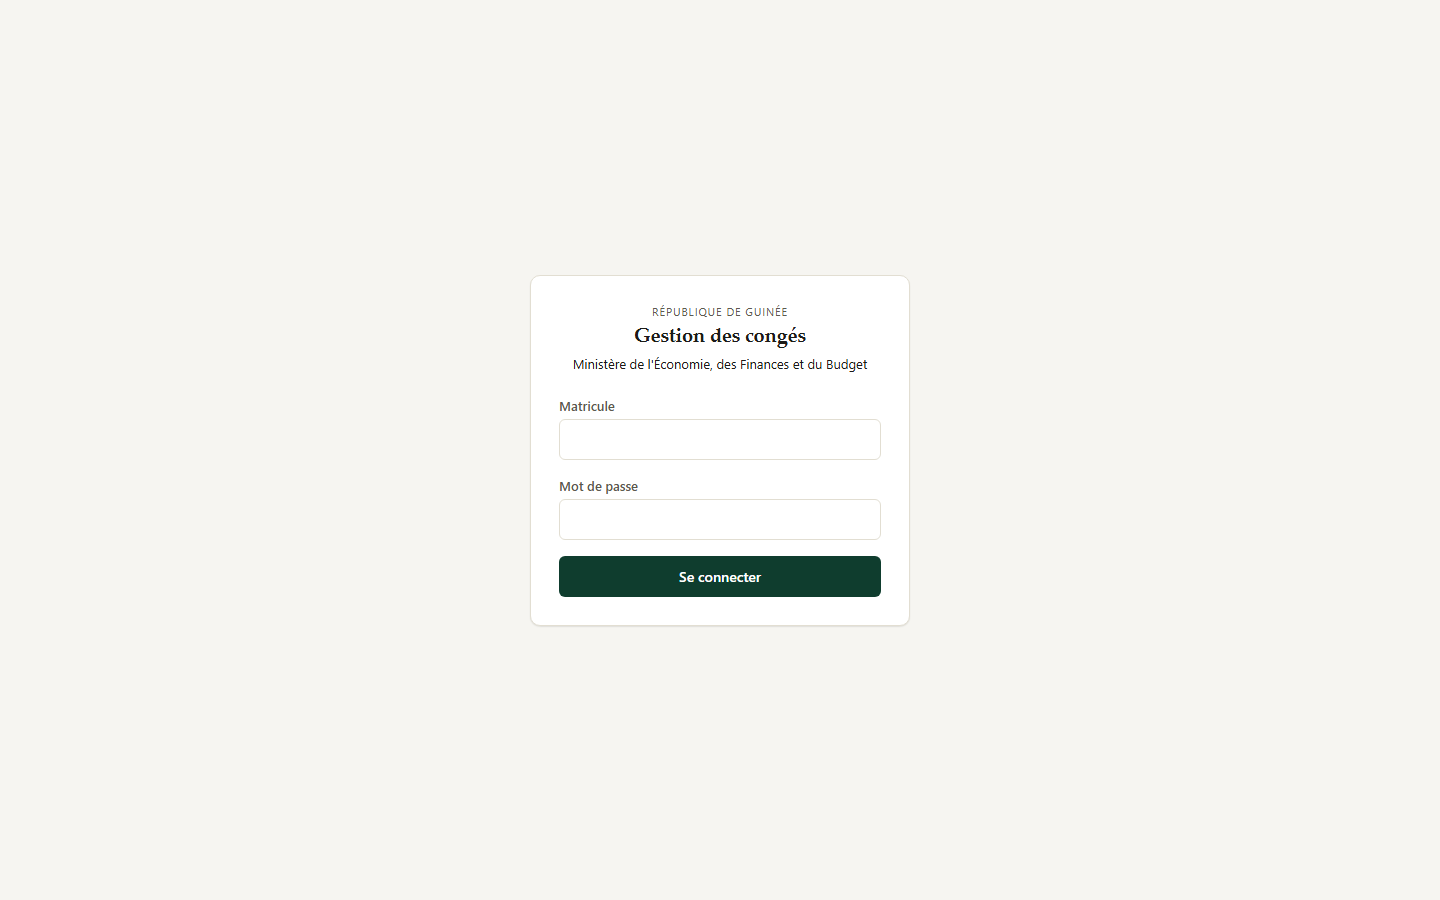
\includegraphics[width=0.55\textwidth]{images/01-connexion.png}
    \caption{Écran de connexion}
    \label{fig:connexion}
\end{figure}

\clearpage
\section{Dépôt d'une demande de congé}

Un agent commence par choisir un type de congé. Le formulaire affiche alors immédiatement la durée attendue et la liste des justificatifs requis pour ce type précis, sans que l'agent ait besoin de les connaître à l'avance.

\begin{figure}[htbp]
    \centering
    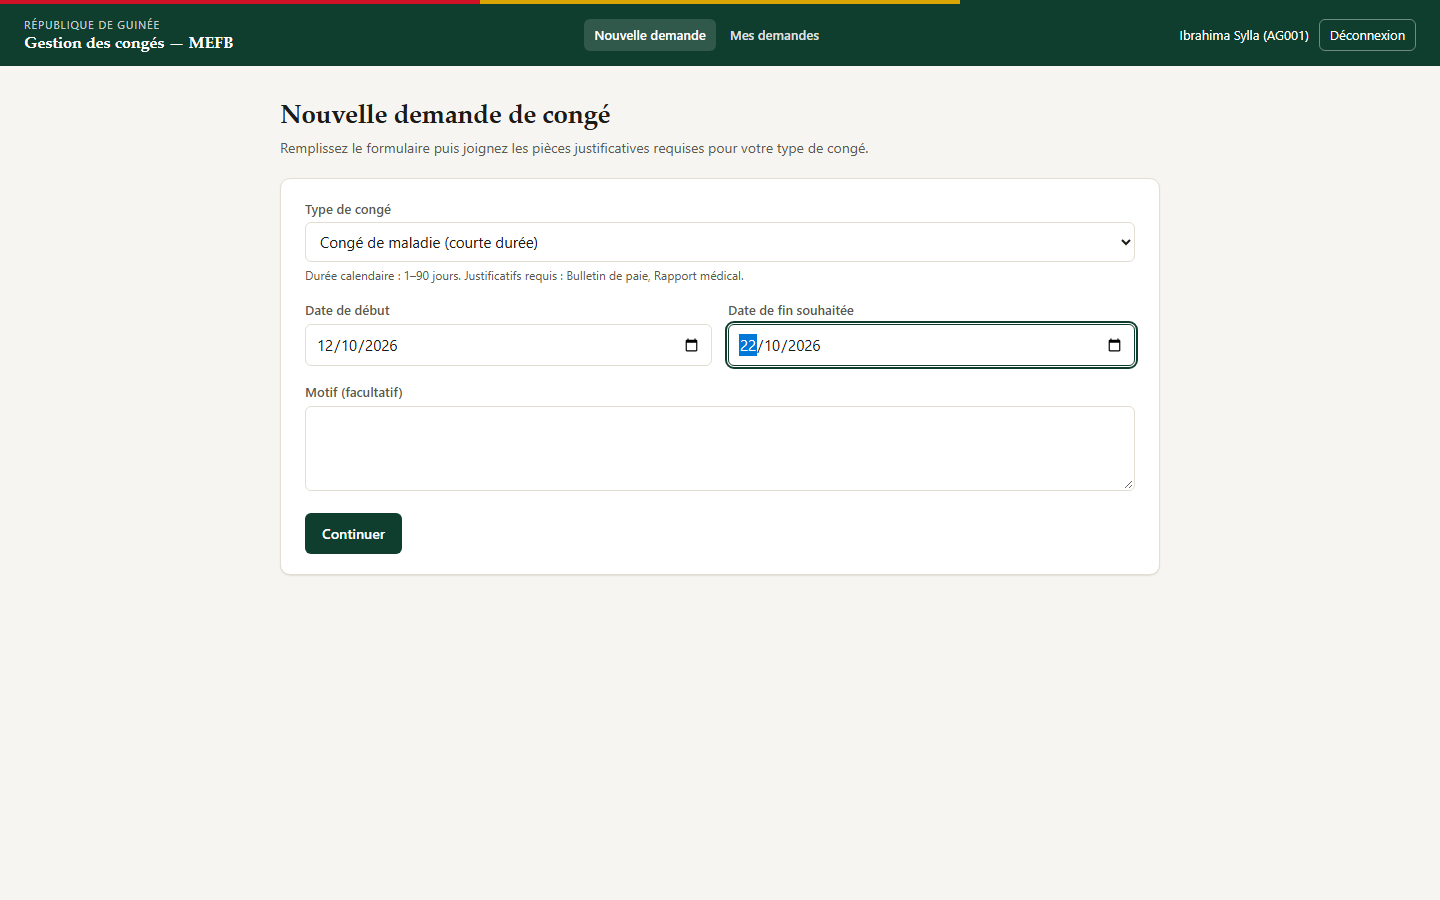
\includegraphics[width=\textwidth]{images/02-nouvelle-demande.png}
    \caption{Formulaire de nouvelle demande, avec les règles du type de congé sélectionné}
    \label{fig:nouvelle-demande}
\end{figure}

Une fois les informations saisies, l'agent est invité à joindre les pièces justificatives correspondantes avant de pouvoir soumettre sa demande. Le bouton de soumission reste désactivé tant qu'un justificatif obligatoire manque.

\begin{figure}[htbp]
    \centering
    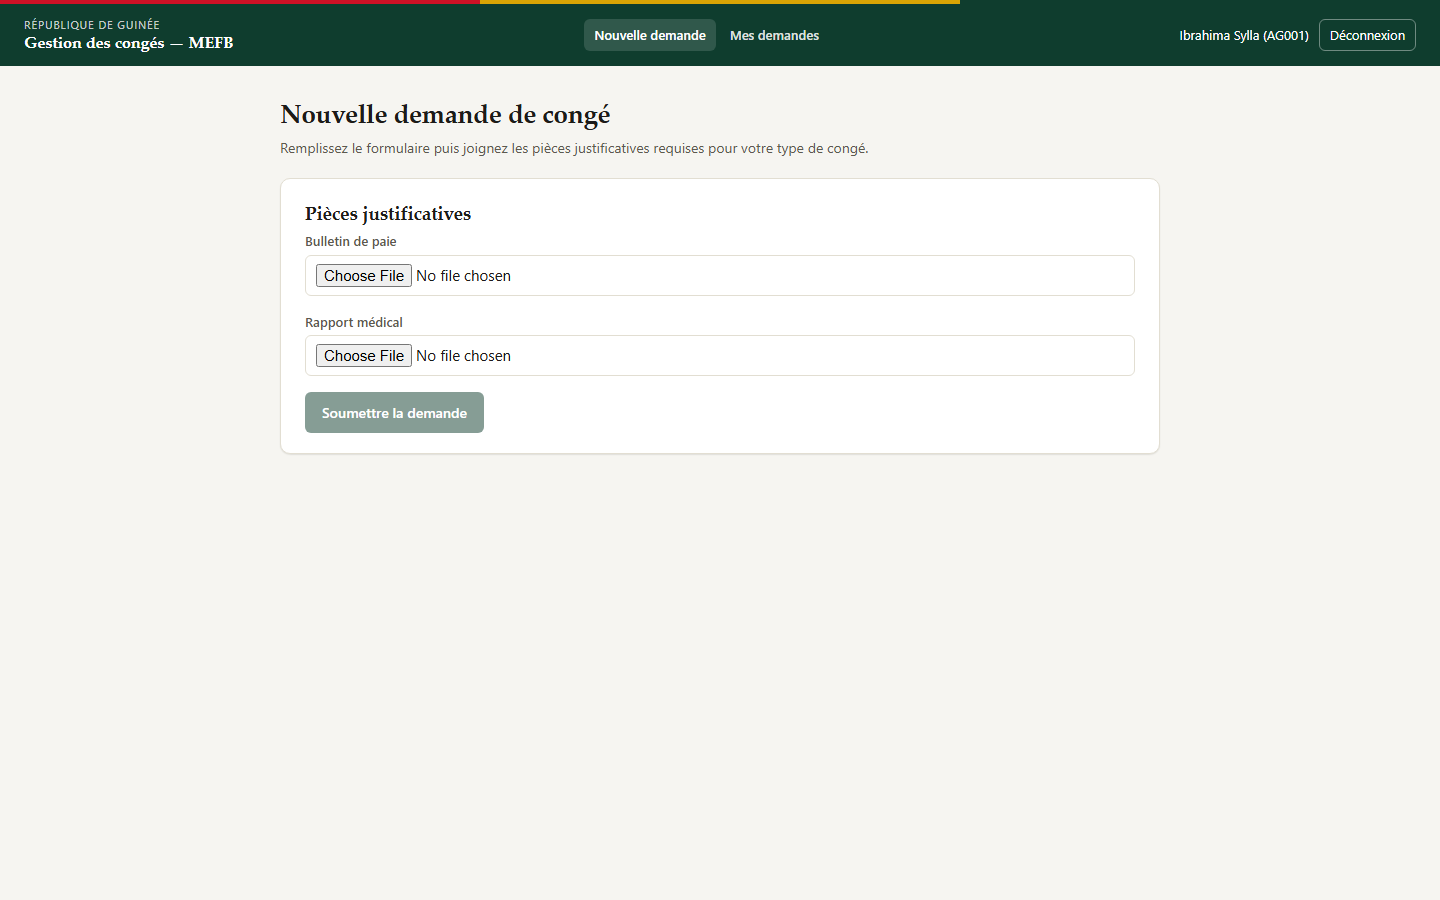
\includegraphics[width=\textwidth]{images/03-justificatifs.png}
    \caption{Dépôt des pièces justificatives requises}
    \label{fig:justificatifs}
\end{figure}

\clearpage
\section{Suivi des demandes}

L'agent retrouve l'historique de ses demandes, avec leur statut à jour, dans un tableau synthétique.

\begin{figure}[htbp]
    \centering
    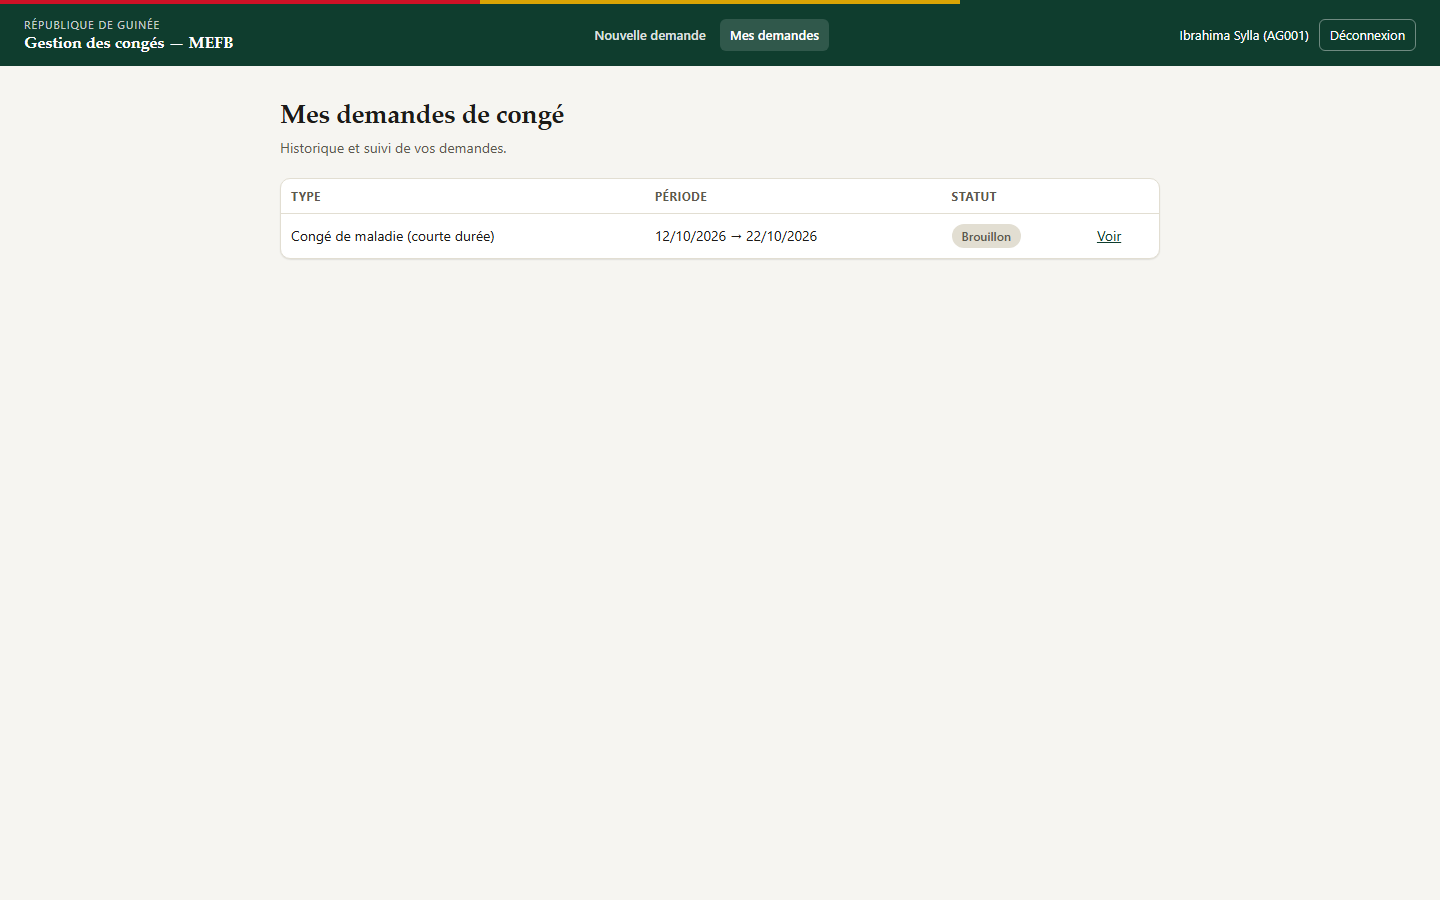
\includegraphics[width=\textwidth]{images/04-mes-demandes.png}
    \caption{Liste des demandes d'un agent}
    \label{fig:mes-demandes}
\end{figure}

En ouvrant une demande, l'agent visualise le détail du circuit de validation en cours, étape par étape, avec le nom du validateur attendu à chaque niveau. Tant qu'aucune décision définitive n'a été prise, il peut également annuler sa demande.

\begin{figure}[htbp]
    \centering
    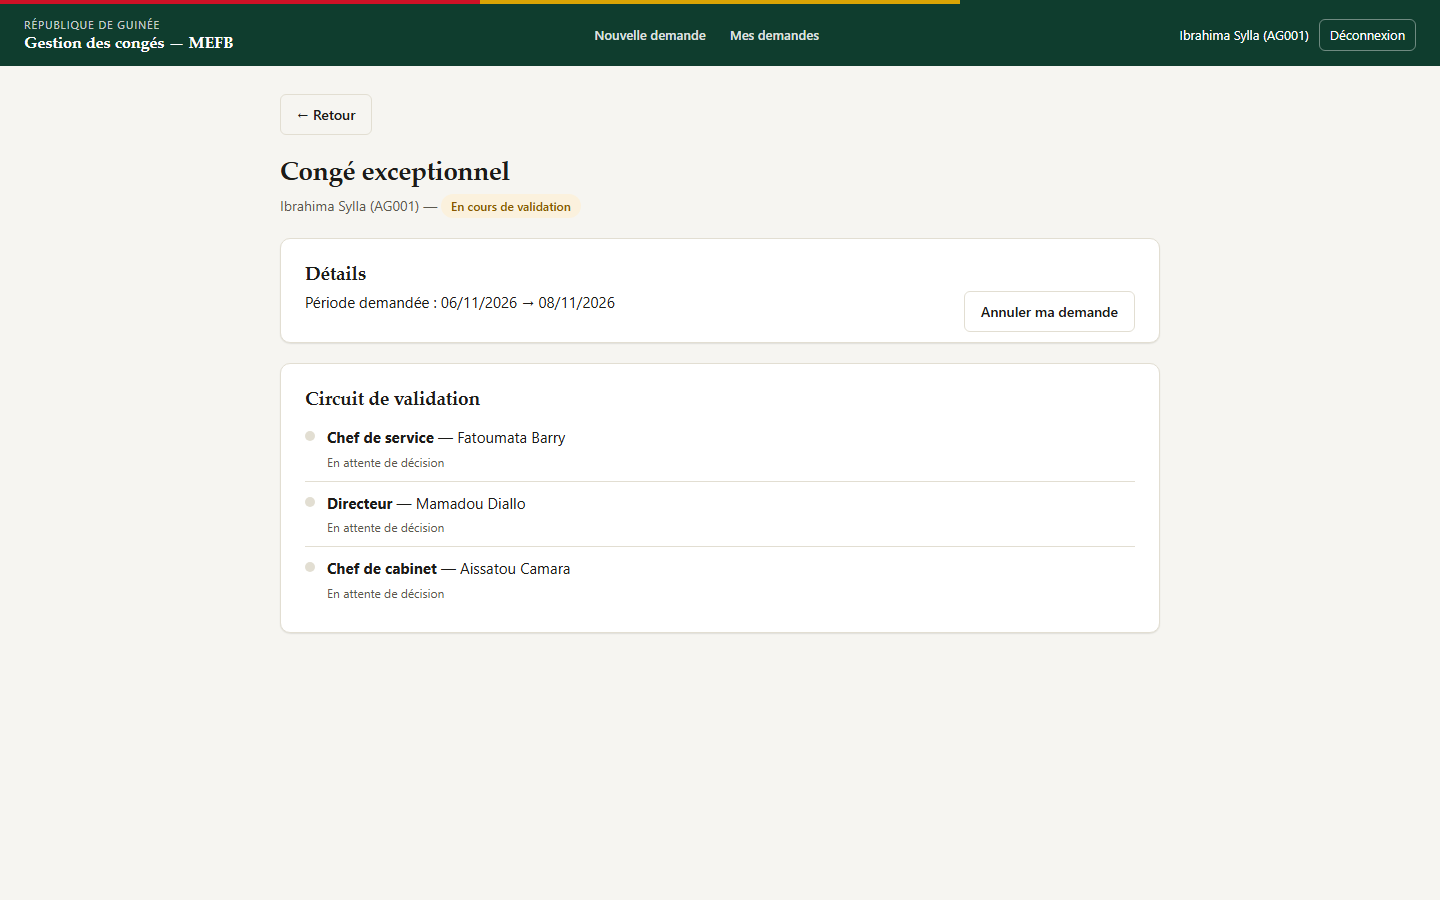
\includegraphics[width=\textwidth]{images/05-detail-demande-en-cours.png}
    \caption{Détail d'une demande en cours de validation}
    \label{fig:detail-demande}
\end{figure}

\clearpage
\section{Validation hiérarchique}

Chaque validateur (chef de service, directeur ou chef de cabinet) dispose d'une file d'attente listant uniquement les demandes qui requièrent effectivement sa décision à l'instant présent.

\begin{figure}[htbp]
    \centering
    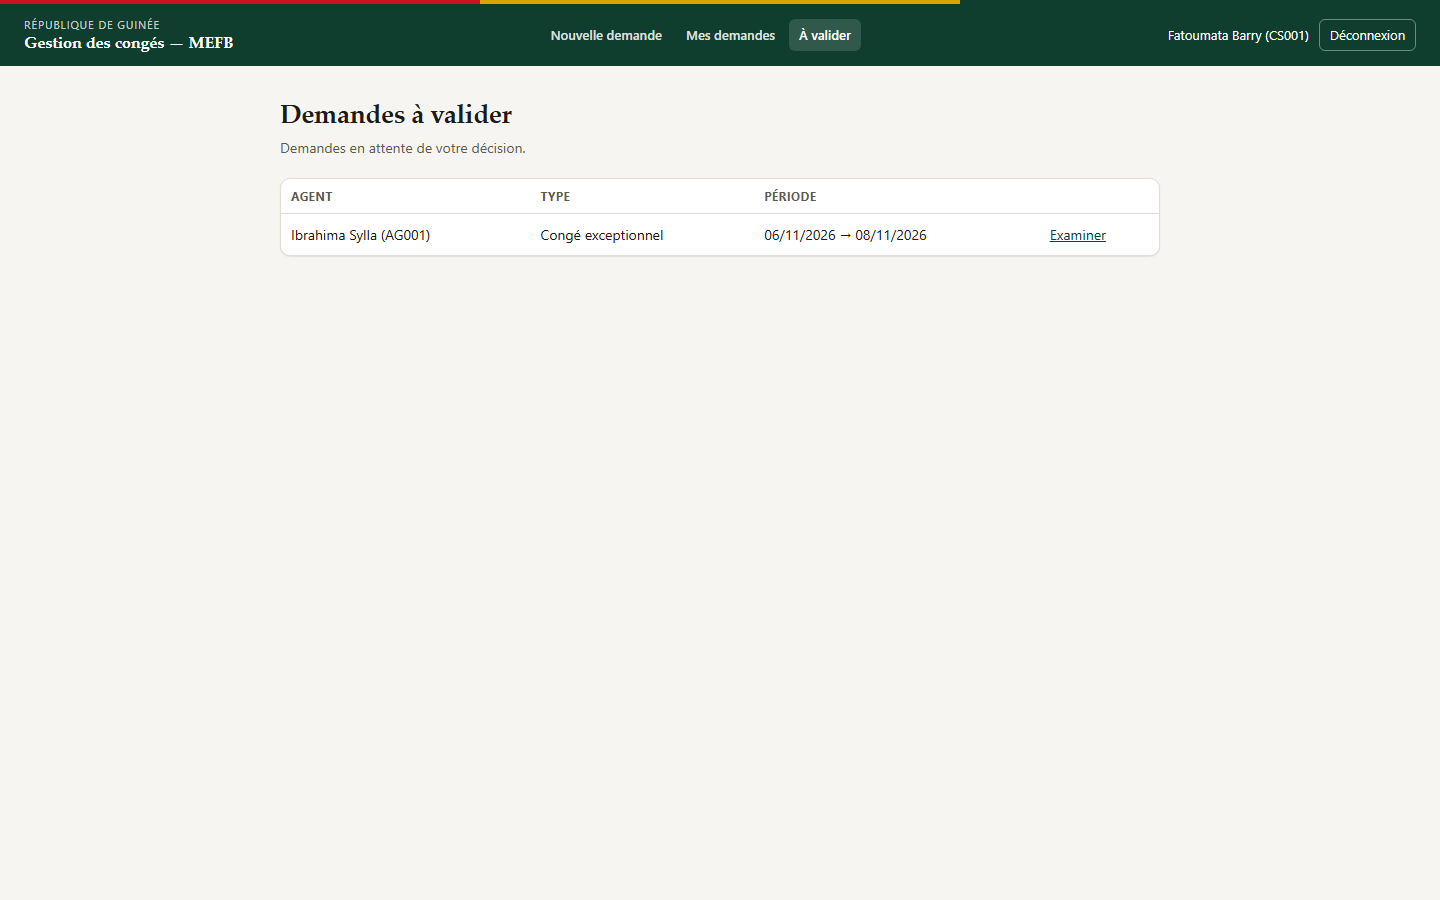
\includegraphics[width=\textwidth]{images/06-a-valider.png}
    \caption{File des demandes à valider}
    \label{fig:a-valider}
\end{figure}

En ouvrant une demande depuis cette file, le validateur retrouve le même circuit que l'agent, complété d'un panneau lui permettant d'approuver ou de rejeter la demande, avec un commentaire obligatoire en cas de rejet.

\begin{figure}[htbp]
    \centering
    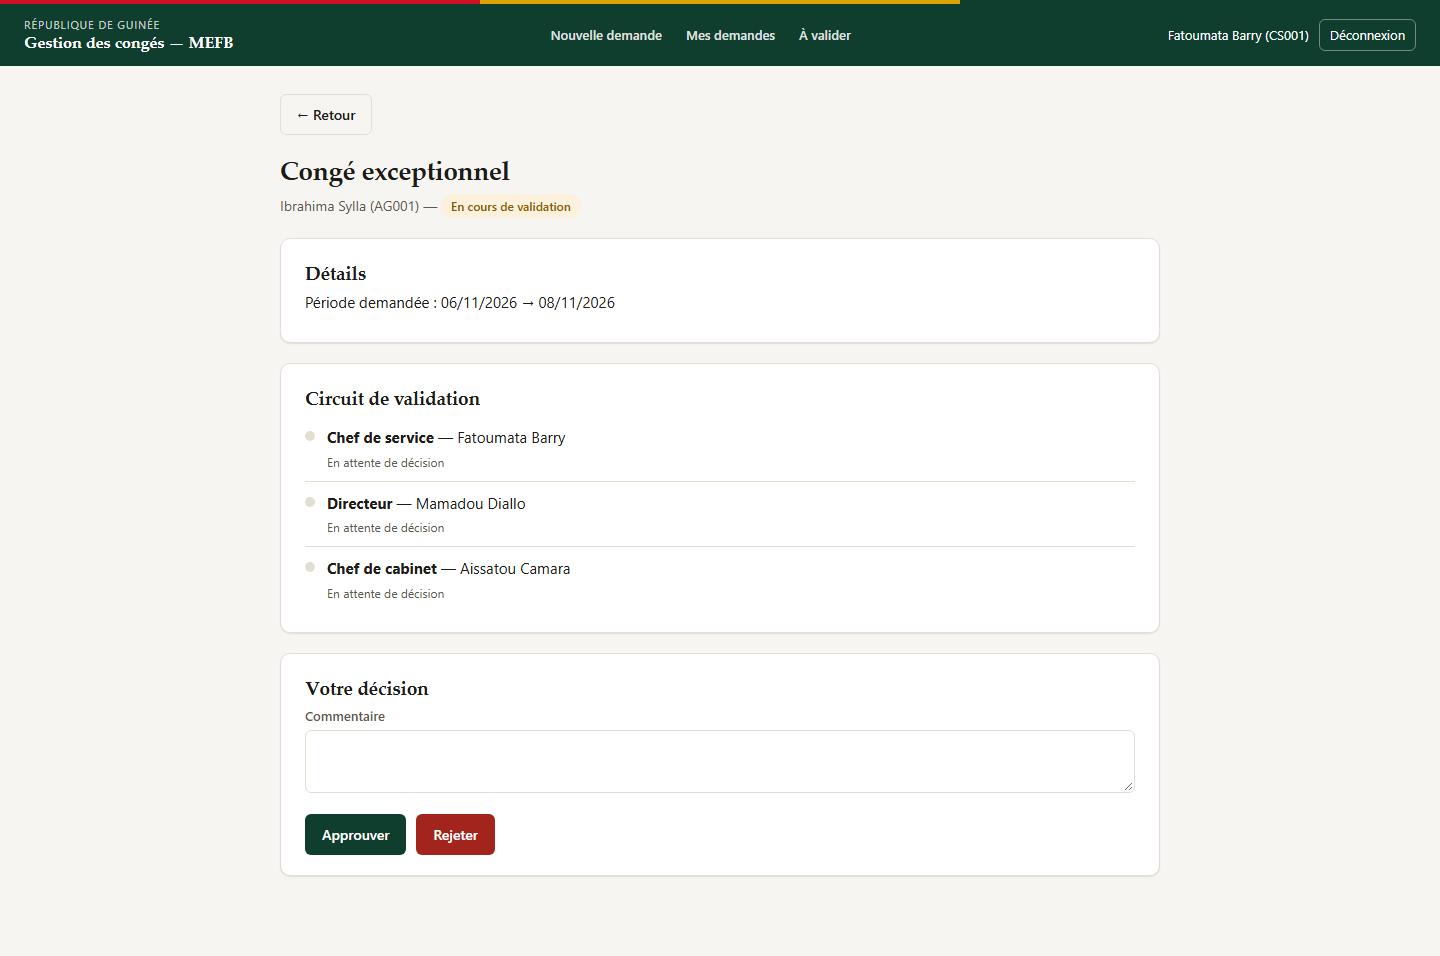
\includegraphics[width=\textwidth]{images/07-decision-validation.png}
    \caption{Prise de décision par un validateur}
    \label{fig:decision-validation}
\end{figure}

\clearpage
\section{Attestation}

Lorsque la dernière étape du circuit est approuvée, l'application génère automatiquement une attestation, immédiatement consultable depuis la demande concernée. Le numéro de série qui y figure permet d'en vérifier l'authenticité de manière indépendante, sans avoir à se connecter à l'application.

\begin{figure}[htbp]
    \centering
    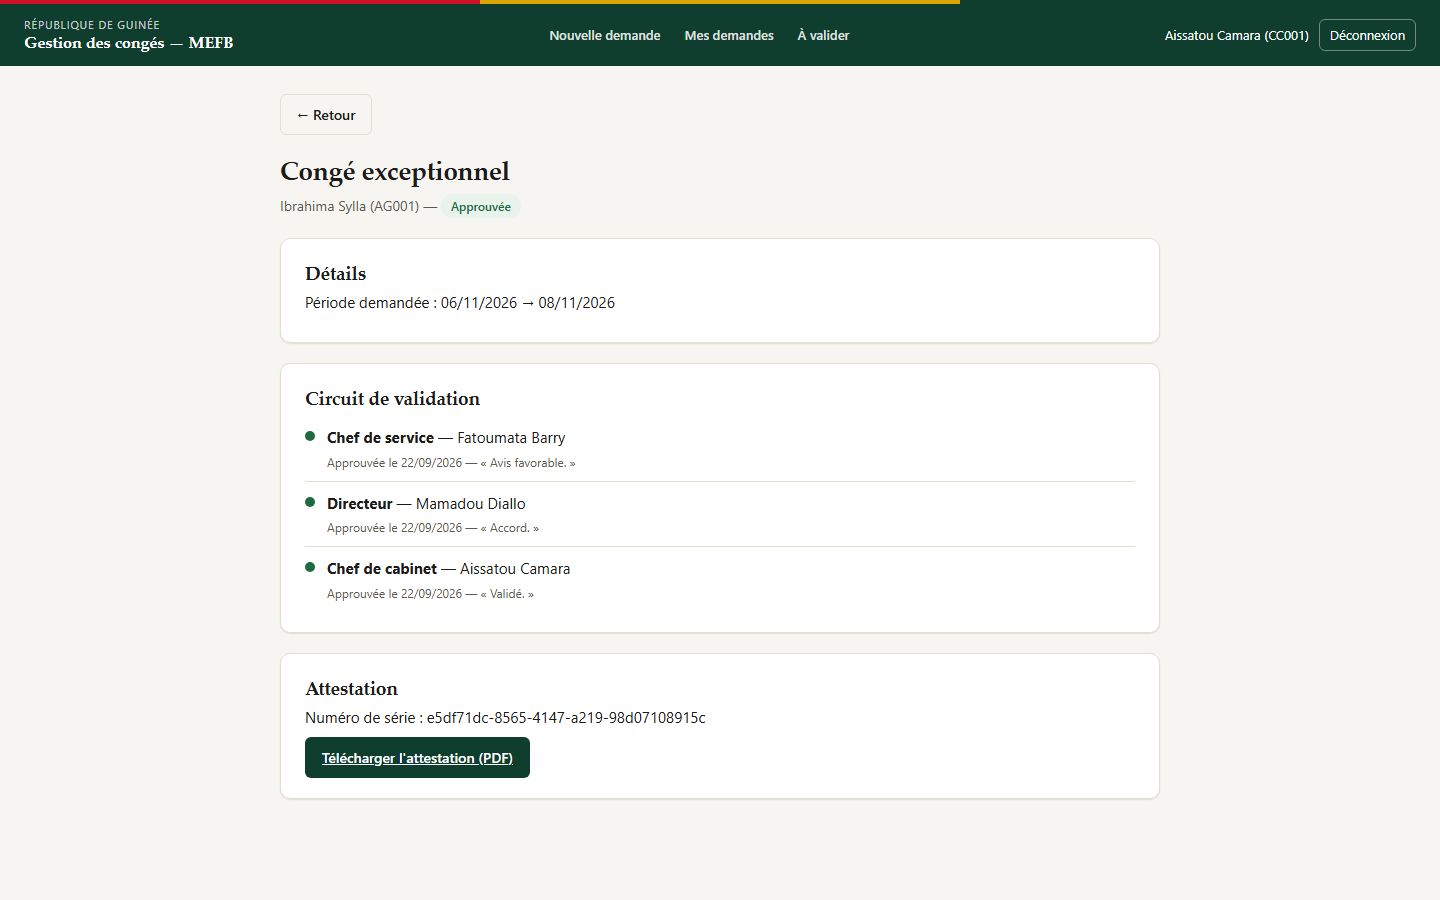
\includegraphics[width=\textwidth]{images/08-attestation-generee.png}
    \caption{Demande approuvée et attestation disponible}
    \label{fig:attestation}
\end{figure}

\clearpage
\section{Administration des comptes et de l'organisation}

Le personnel des ressources humaines dispose d'écrans dédiés pour créer les comptes des agents et gérer la structure organisationnelle du ministère, dont dépend directement le calcul du circuit de validation de chaque demande.

\begin{figure}[htbp]
    \centering
    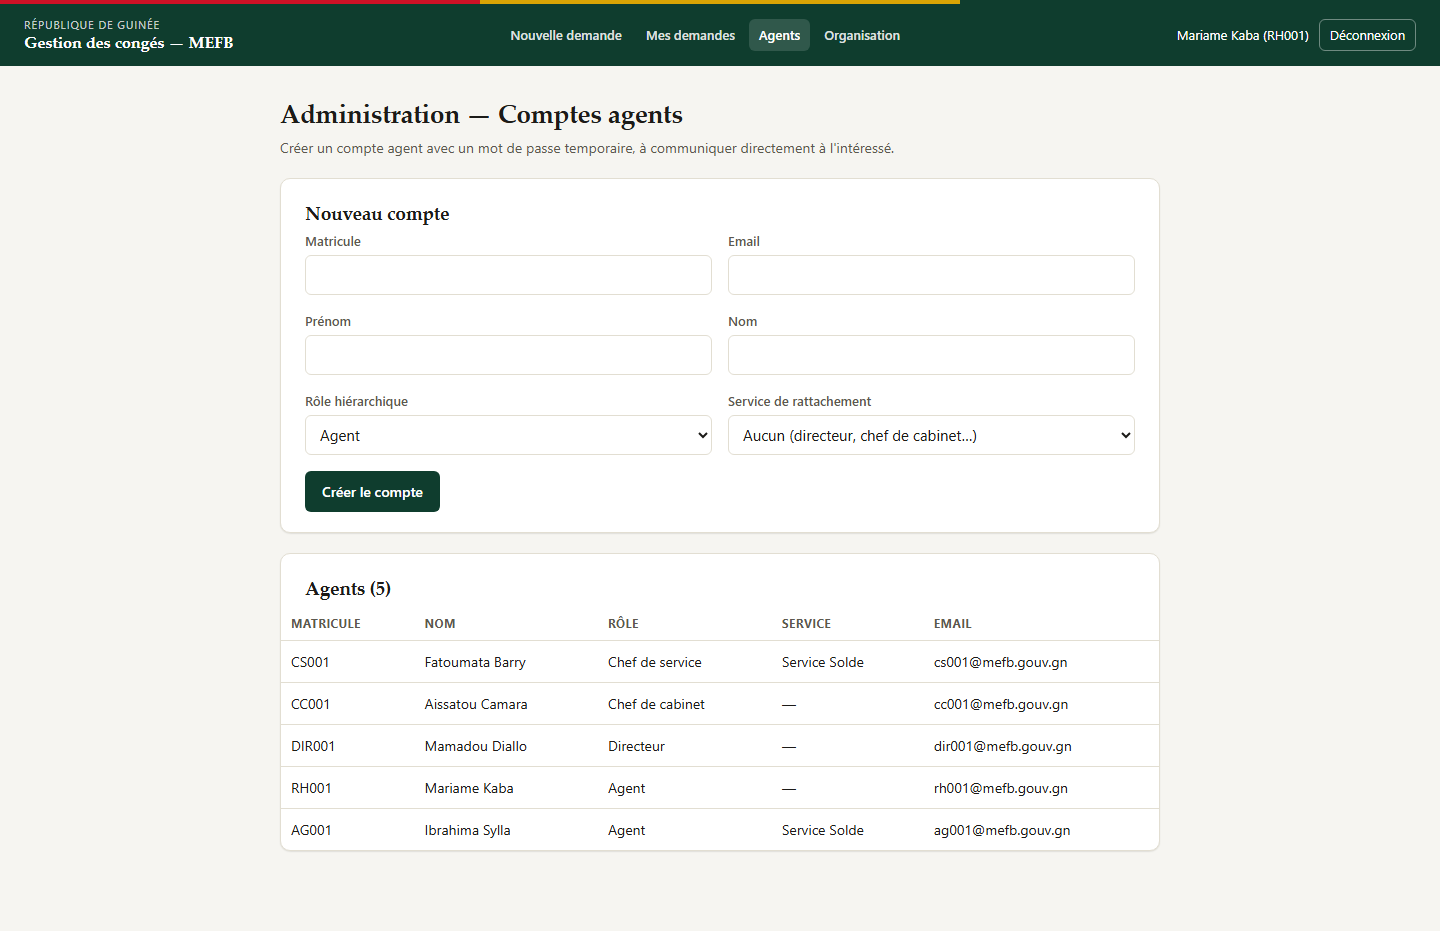
\includegraphics[width=\textwidth]{images/09-administration-agents.png}
    \caption{Création et consultation des comptes agents}
    \label{fig:administration-agents}
\end{figure}

\begin{figure}[htbp]
    \centering
    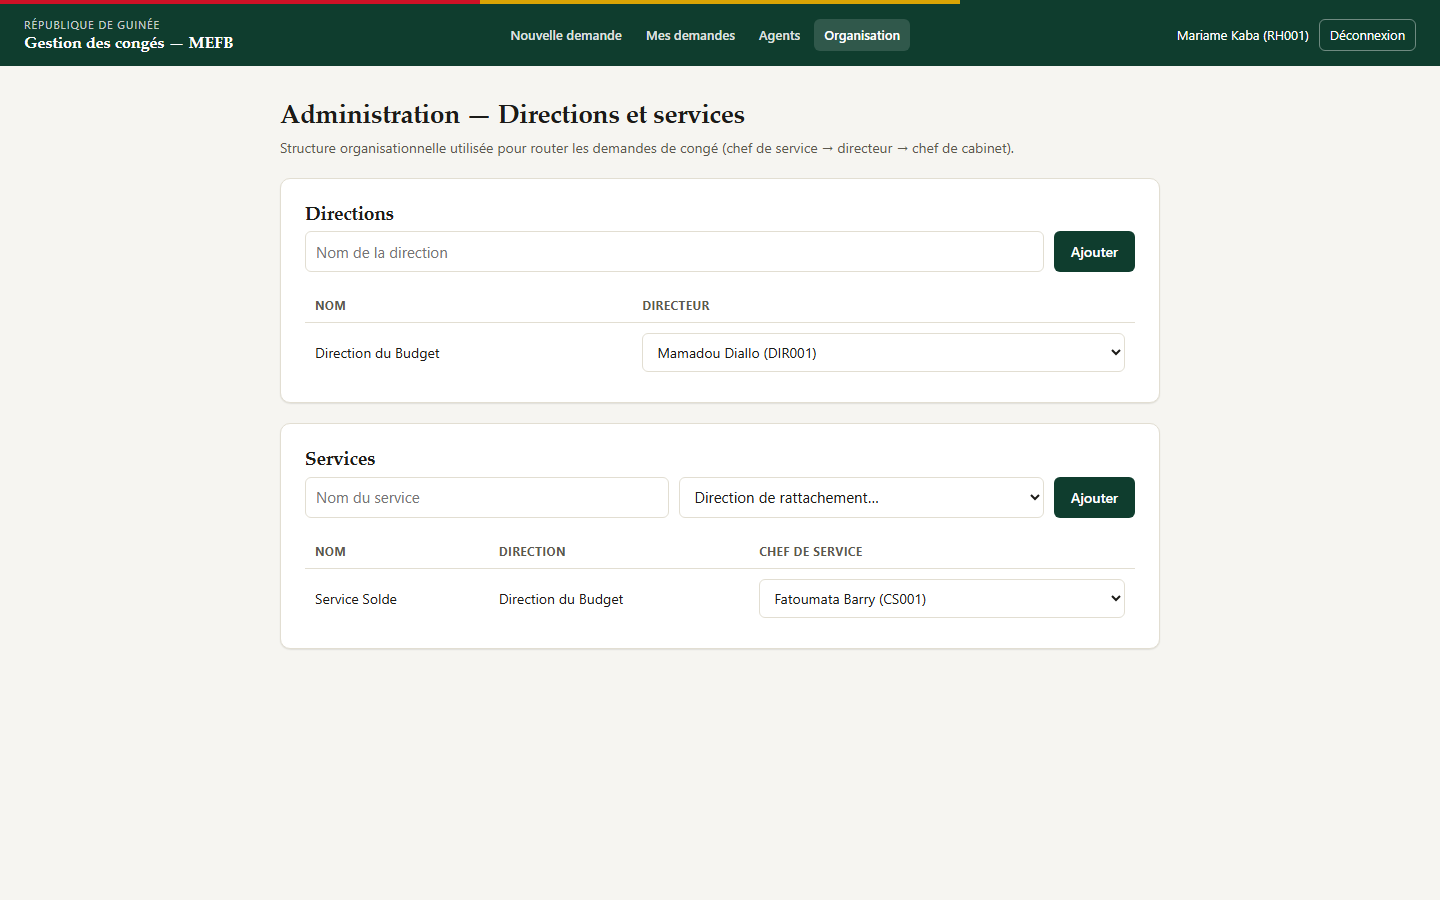
\includegraphics[width=\textwidth]{images/10-administration-organisation.png}
    \caption{Gestion des directions et des services}
    \label{fig:administration-organisation}
\end{figure}

%   \input{chapters/tests-et-difficultes}
%   \input{chapters/conclusion}

\end{document}
